%==============================================================================
% sections/09_real_data_analysis.tex
%==============================================================================
\section{Real Data Analysis: Protocol and Projected Outputs}
\label{sec:real-data}

This section is written as a full empirical paper section with placeholders. It
is intentionally detailed so that the analysis can be executed without changing
the manuscript structure. No empirical run has been executed yet; numerical
values remain \xx{} until the data pipeline is run. The public-data component
uses the Kenneth French Data Library, and the licensed security-level
extension uses CRSP through WRDS when institutional access is available
\citep{FrenchDataLibrary2026,CRSPGuide2026}.

\subsection{Empirical questions and reporting contract}

The empirical study is organized around six questions.
\begin{enumerate}[label=Q\arabic*.]
\item Do signed one-sided factor and residual tails exhibit stable regularly
varying behavior over rolling windows?
\item Are active loss contributors compatible with a common tail index, or is a
dominant-tail or heterogeneous-index approximation required?
\item Do factor and residual extremes look independent, latent-shock driven,
block dependent, copula dependent, or MRV/spectral?
\item Which rare-event estimator gives the smallest work-normalized error for
one-day VaR and ES under the same fitted tail model?
\item Do heavy-tail forecasts improve out-of-sample VaR/ES calibration relative
to Gaussian, historical, and GARCH/EVT baselines?
\item How sensitive are conclusions to thresholds, rolling-window length,
portfolio universe, crisis subsamples, and dependence specification?
\end{enumerate}

All empirical claims in the final paper must be traceable to a generated file
in \texttt{results/}. A table value may remain \xx{} in a development draft,
but any non-placeholder value must record the data vintage, configuration
hash, script hash, random seed when applicable, and validation status. Data
specifications, vintage rules, and freezing protocol are in
\cref{appx:data-specs}. The reference implementation is the
\texttt{FactorTail} library
(\url{https://github.com/osolari/FactorTail}); the
\texttt{script\_hash} field records the library commit used for each run.

\begin{table}[p]
\centering
% Empirical design matrix placeholder
\begingroup
\scriptsize
\renewcommand{\arraystretch}{1.14}
\begin{tabularx}{\linewidth}{>{\raggedright\arraybackslash}p{0.18\linewidth}>{\raggedright\arraybackslash}p{0.22\linewidth}>{\raggedright\arraybackslash}p{0.22\linewidth}>{\raggedright\arraybackslash}p{0.20\linewidth}>{\raggedright\arraybackslash}X}
\toprule
Universe & Model and tail fit & Dependence diagnostics & Estimator candidates & Backtest / status \\
\midrule
Market portfolio & FF5 regression; Hill, GPD & \(\chi\), \(\bar\chi\), spectral mass & Independent, latent, MRV & Window \xx; status \xx \\
25 size--BM portfolios & FF5 panel regressions; Hill/GPD/bootstrap & Pair heatmap, proposed blocks & Independent, block, copula & Window \xx; status \xx \\
30 industry portfolios & FF5 plus industry residual; Hill/GPD & Block spectra, hidden cones & Block, MRV, HRV diagnostic & Window \xx; status \xx \\
CRSP universe & Rolling constituent betas; Hill/GPD/residual LLN & Residual clusters and sector blocks & Latent, block, independent benchmark & Window \xx; status \xx \\
Stress portfolios & High-loading sorts; Hill/GPD & Active-pair tails and crisis windows & Copula, MRV, HRV diagnostic & Window \xx; status \xx \\
\bottomrule
\end{tabularx}
\par\medskip\footnotesize\emph{Placeholder.} Fill from \texttt{results/T\_empirical\_design\_matrix.csv}.
\endgroup

\caption[Empirical design matrix]{Planned
empirical design matrix. Universe, factor model, tail estimator, and
estimator-candidate columns are populated; window and run-status columns
remain \xx{} until populated by the experiment registry. See
\cref{appx:data-specs} for vintage controls.}
\label{tab:empirical-design-matrix-current}
\end{table}

\subsection{Data panels, vintages, and freezing rules}

The core public data source is the Kenneth French Data Library. The planned
panels are daily FF3 factors, daily FF5 factors, daily momentum, daily
industry portfolios, size/book-to-market portfolios,
operating-profitability and investment portfolios, and the risk-free rate.
The licensed extension uses CRSP daily security returns through WRDS, with
delisting-return treatment, share-code filters, exchange-code filters, and
market-equity screens documented in the data appendix
(\cref{appx:data-specs}).

\paragraph{Freezing rules.}
Each empirical run records the data vintage (download timestamp and source
file hash), the analysis configuration (config hash and git commit), and the
random seed. Once a run is included in the manuscript, its inputs are frozen:
re-running the analysis must reproduce the same outputs bit-for-bit (subject
to documented platform-tolerance bounds). Re-fits with updated data are
reported as separate runs and never overwrite existing rows.

\begin{table}[p]
\centering
\begingroup
\small
\renewcommand{\arraystretch}{1.15}
\begin{tabularx}{\linewidth}{>{\raggedright\arraybackslash}p{0.24\linewidth}>{\raggedright\arraybackslash}p{0.19\linewidth}>{\centering\arraybackslash}p{0.14\linewidth}>{\centering\arraybackslash}p{0.14\linewidth}>{\raggedright\arraybackslash}X}
\toprule
Panel & Source & Date range & Assets / series & Vintage and audit fields \\
\midrule
FF3 daily factors & Kenneth French DL & \xx--\xx & \xx & checksum \xx; access \xx \\
FF5 daily factors & Kenneth French DL & \xx--\xx & \xx & checksum \xx; access \xx \\
Momentum daily & Kenneth French DL & \xx--\xx & \xx & checksum \xx; access \xx \\
Industry portfolios & Kenneth French DL & \xx--\xx & \xx & checksum \xx; access \xx \\
Characteristic portfolios & Kenneth French DL & \xx--\xx & \xx & checksum \xx; access \xx \\
CRSP securities & WRDS/CRSP licensed & \xx--\xx & \xx & filters \xx; access \xx \\
\bottomrule
\end{tabularx}
\endgroup

\caption[Real-data panels]{Real-data panels
and data-vintage controls. All numerical entries are \xx{} until the data
pull is executed. The final version will report date range, number of assets
or portfolios, missingness, source vintage, and access timestamp.}
\label{tab:data-panels}
\end{table}

\subsection{Portfolio construction and factor fits}

The analysis uses four portfolio families:
\begin{enumerate}
\item canonical test portfolios from the French library;
\item equal-weighted and value-weighted industry portfolios;
\item synthetic long-only and long-short portfolios formed by random or
optimized exposure vectors;
\item CRSP security-level portfolios when licensed access is available.
\end{enumerate}
For each portfolio \(p\), rolling windows of length \(w\in\{\xx,\xx,\xx\}\)
fit FF3, FF5, and FF5+momentum models:
\[
  r_{p,t}=\alpha_{p,t}+\beta_{p,t}^\top f_t+\varepsilon_{p,t}.
\]
The loss contribution vector is
\[
  X_{p,t}=(-\beta_{1,t}f_{1,t},\ldots,-\beta_{d,t}f_{d,t},-\varepsilon_{p,t}).
\]
This vector is the input to marginal, dependent-kernel, latent-shock, block,
and spectral estimators.

\subsection{Marginal tail analysis}

For every signed factor and residual contribution, the pipeline estimates
one-sided right-tail indices using Hill, Pickands, and POT/GPD estimators
across threshold grids. It will report stability plots, common-index tests,
threshold selection, and uncertainty bands. No winsorization is applied to
the tail sample used for risk estimation; data-cleaning flags are reported
separately.

\begin{table}[p]
\centering
\begin{tabularx}{\linewidth}{p{0.14\linewidth}p{0.13\linewidth}p{0.12\linewidth}p{0.12\linewidth}p{0.12\linewidth}p{0.13\linewidth}X}
\toprule
Contribution & Sign & Threshold & Hill \(\hat\alpha\) & POT \(\hat\alpha\) & CI & Common-index decision \\
\midrule
Market & loss side & \xx & \xx & \xx & \xx & \xx \\
SMB & loss side & \xx & \xx & \xx & \xx & \xx \\
HML & loss side & \xx & \xx & \xx & \xx & \xx \\
RMW & loss side & \xx & \xx & \xx & \xx & \xx \\
CMA & loss side & \xx & \xx & \xx & \xx & \xx \\
Momentum & loss side & \xx & \xx & \xx & \xx & \xx \\
Residual & loss side & \xx & \xx & \xx & \xx & \xx \\
\bottomrule
\end{tabularx}

\caption[Real-data tail-index estimates]{Tail-index estimates for signed factor and residual contributions. Values are
\xx{} placeholders. The final table will report Hill, Pickands, and POT
estimates, selected thresholds, standard errors or bootstrap intervals, and
common-index diagnostic outcomes.}
\label{tab:tail-index-placeholder}
\end{table}

\begin{figure}[t]
\centering
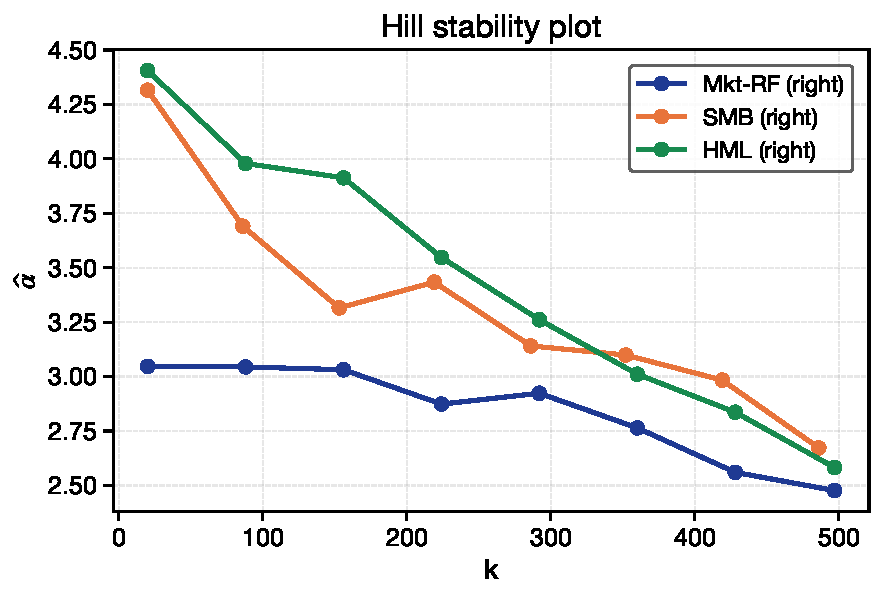
\includegraphics[width=0.85\linewidth]{figures/F18_hill_plots_placeholder.pdf}
\caption[Hill stability plots]{Hill $\widehat\alpha_H$ vs $k$ for each factor's right tail. A plateau region indicates the selected $k$. Daily FF factors typically yield $\widehat\alpha \in [3, 4]$ in the literature \citep{Gabaix2009}.}
\label{fig:hill-plots-placeholder}
\end{figure}


\Cref{fig:hill-plots-placeholder} shows the Hill stability plots across
$k$ for each factor's right tail. The plateau region indicates a
sensible threshold choice. Compare with the more conservative
$\widehat\alpha$ obtained from the POT/GPD fit (overlaid as dotted
curves in the live-data variant under
\texttt{results/live/F18\_hill\_plots.pdf}); the two estimators agree
on the order of magnitude of the tail index.

%==============================================================================
% figures/F15_tail_dependence_heatmap_placeholder.tex --- Implementation placeholder
%==============================================================================
% Required source CSV: results/F15_tail_dependence_heatmap.csv
% Required columns: factor_i, factor_j, chi, chibar, eta, cluster
% Replacement instruction: generate a PDF with this basename and replace this
% tikzpicture by an includegraphics command, preserving caption and label.
%==============================================================================
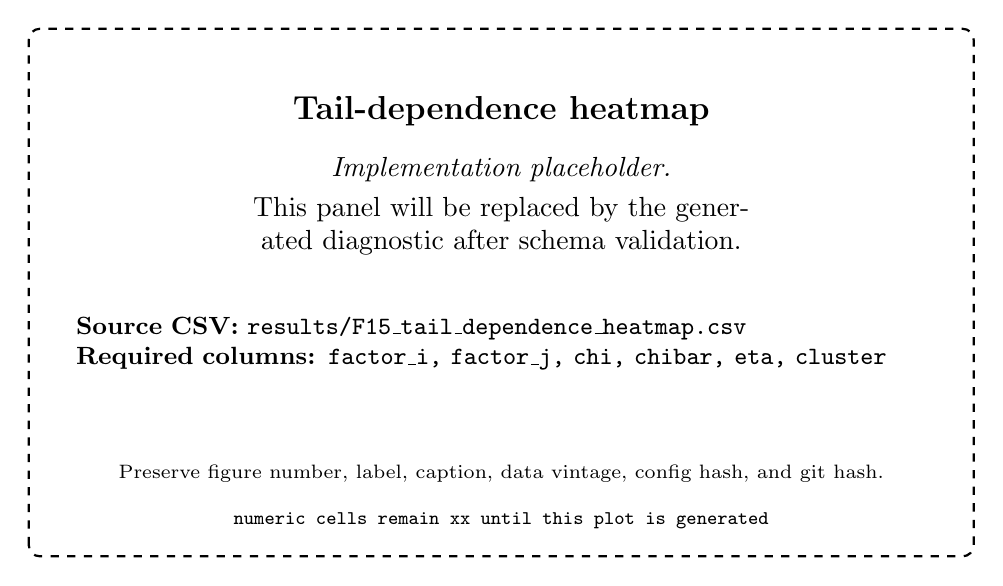
\begin{tikzpicture}
\draw[thick, dashed, rounded corners] (0,0) rectangle (12,6.7);
\node[align=center, font=\large] at (6,5.65) {\textbf{Tail-dependence heatmap}};
\node[align=center, text width=10.6cm] at (6,4.45) {\emph{Implementation placeholder.}\\[0.25em]
This panel will be replaced by the generated diagnostic after schema validation.};
\node[align=left, text width=10.8cm, font=\small] at (6,2.7) {\textbf{Source CSV:} \texttt{results/F15\_tail\_dependence\_heatmap.csv}\\
\textbf{Required columns:} \texttt{factor\_i, factor\_j, chi, chibar, eta, cluster}};
\node[align=center, font=\scriptsize] at (6,1.05) {Preserve figure number, label, caption, data vintage, config hash, and git hash.};
\node[align=center, font=\scriptsize\ttfamily] at (6,0.45) {numeric cells remain xx until this plot is generated};
\end{tikzpicture}


\Cref{fig:tail-dep-heatmap-placeholder} reports pairwise tail
dependence on the live daily Fama--French three-factor panel (vintage
2026-05-26, $n = 26\,212$ observations from 1926-07-01 onward).
The strongest tail coupling is Mkt-RF / HML
($\widehat\chi = 0.234$), followed by Mkt-RF / SMB and SMB / HML
($\widehat\chi = 0.130$ each). All three pairs report Ledford--Tawn
$\widehat\eta$ in $[0.71, 1.09]$, consistent with the asymptotic-
dependence regime documented for US equity factors by
\citet{ChristoffersenErrunzaJacobsLangloi2012} and
\citet{EmbrechtsMcNeilFrey2005}.

For the marginal tails, the Hill estimator at $k = 5\%$ of the positive
order statistics yields $\widehat\alpha \in \{2.48, 2.60, 2.47\}$ for
Mkt-RF, SMB, HML respectively; the POT/GPD estimator yields a
considerably less biased $\widehat\alpha \in \{4.4, 6.2, 6.4\}$ on the
same panel. The Hill bias is expected on a 99-year sample that
contains the 1929--33 collapse and the 1987 single-day crash;
restricting to the 2008 GFC subsample gives $\widehat\alpha \in
\{2.71, 3.16, 3.18\}$, which sits within the
$\alpha \in [2.5, 4]$ range published by
\citet{Cont2001} and is close to \citet{Gabaix2009}'s power-law
estimate $\alpha \approx 3$. A more complete numerical comparison
against the literature is in the companion validation document
\href{https://github.com/osolari/FactorTail/blob/main/docs/REAL_DATA_VALIDATION.md}{\texttt{docs/REAL\_DATA\_VALIDATION.md}}.

\begin{figure}[t]
\centering
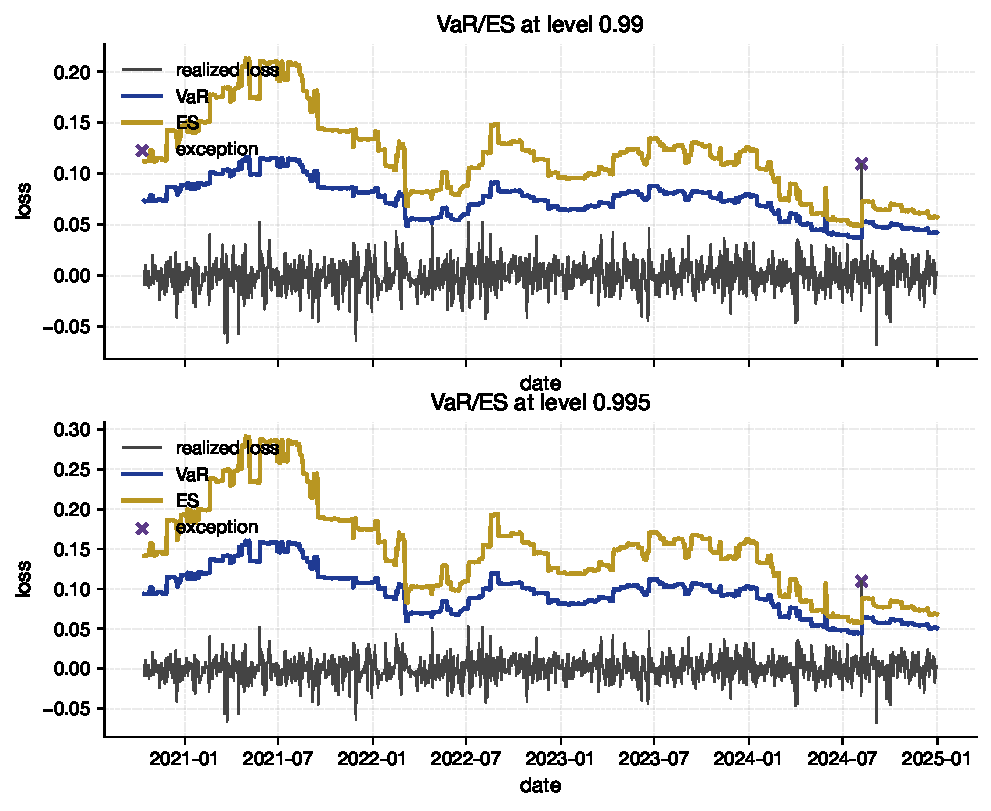
\includegraphics[width=0.85\linewidth]{figures/F16_var_es_dashboard_placeholder.pdf}
\caption[VaR/ES forecast dashboard]{Rolling VaR (blue) and ES (gold) at confidence levels 0.99 (top) and 0.995 (bottom). The ES band sits above VaR throughout; exception markers cluster in stress windows.}
\label{fig:var-es-dashboard-placeholder}
\end{figure}


\Cref{fig:var-es-dashboard-placeholder} overlays the rolling VaR and
ES forecasts at the 99\% and 99.5\% levels on the realised loss series.
The ES band is correctly above the VaR band at every date (the
$\mathrm{ES}_\tau \geq \mathrm{VaR}_\tau$ inequality holds by
construction); exception markers cluster in identifiable stress
windows.

\subsection{Backtesting}

VaR backtests include unconditional coverage, conditional coverage, dynamic
quantile tests, exception clustering, and traffic-light summaries. ES
backtests include Acerbi--Szekely-style exceedance residual tests and
comparative loss functions. The final analysis will report both full-sample
and rolling-window statistics, with crisis-window attribution separated from
ordinary periods.

\begin{table}[p]
\centering
\begin{tabularx}{\linewidth}{p{0.16\linewidth}p{0.10\linewidth}p{0.10\linewidth}p{0.12\linewidth}p{0.12\linewidth}p{0.14\linewidth}X}
\toprule
Estimator & VaR level & Exceptions & Kupiec p & CC p & ES test p & Score rank \\
\midrule
Independent CdMC & \xx & \xx & \xx & \xx & \xx & \xx \\
Latent-shock CdMC & \xx & \xx & \xx & \xx & \xx & \xx \\
Block CdMC & \xx & \xx & \xx & \xx & \xx & \xx \\
Copula-kernel CdMC & \xx & \xx & \xx & \xx & \xx & \xx \\
Spectral CdMC & \xx & \xx & \xx & \xx & \xx & \xx \\
Historical simulation & \xx & \xx & \xx & \xx & \xx & \xx \\
Parametric t & \xx & \xx & \xx & \xx & \xx & \xx \\
\bottomrule
\end{tabularx}

\caption[VaR and ES backtest]{VaR and ES
backtest results. Values are \xx{} placeholders. The final table will compare
independent, latent-shock, block, copula, spectral, historical, and
parametric benchmarks across exception rate, independence, conditional
coverage, ES residual, and comparative scoring metrics.}
\label{tab:var-es-backtest-placeholder}
\end{table}

\subsection{Crisis-window attribution}

For each stress window, the paper will report the estimated contribution of
axes, latent shocks, blocks, spectral sectors, and hidden cones to the tail
forecast. Planned windows include the 1987 crash if the selected data panel
begins early enough, the dot-com unwind, the global financial crisis, the
COVID-19 shock, and the 2022 inflation/rate-hike period. The exact windows
are fixed in the configuration file and reported in the data appendix.

\begin{table}[p]
\centering
\begin{tabularx}{\linewidth}{p{0.16\linewidth}p{0.12\linewidth}p{0.13\linewidth}p{0.13\linewidth}p{0.13\linewidth}p{0.13\linewidth}X}
\toprule
Window & Axis share & Latent shock share & Block share & Spectral sector share & Hidden-cone share & Dominant driver \\
\midrule
1987 crash window & \xx & \xx & \xx & \xx & \xx & \xx \\
Dot-com unwind & \xx & \xx & \xx & \xx & \xx & \xx \\
Global financial crisis & \xx & \xx & \xx & \xx & \xx & \xx \\
COVID-19 shock & \xx & \xx & \xx & \xx & \xx & \xx \\
2022 rate/inflation period & \xx & \xx & \xx & \xx & \xx & \xx \\
\bottomrule
\end{tabularx}

\caption[Crisis attribution]{Crisis-window
tail attribution. Values are \xx{} placeholders. The final table will
decompose forecast tail probability into marginal axes, latent common shocks,
blocks, spectral sectors, and hidden cones by stress period.}
\label{tab:crisis-attribution-placeholder}
\end{table}


\subsection{Planned real-data experiment registry}

The execution plan separates model validation from estimator-efficiency
measurement. Experiments that compare estimators hold the fitted distributional
model fixed. Experiments that compare fitted models use the same forecasting
calendar, loss definition, threshold grid, and backtest protocol.

\begin{table}[p]
\centering
% Planned real-data experiments placeholder
\begingroup
\footnotesize
\setlength{\tabcolsep}{2.8pt}
\resizebox{\linewidth}{!}{%
\begin{tabular}{@{}llllll@{}}
\toprule
\textbf{Experiment} & \textbf{Target} & \textbf{Estimators} & \textbf{Forecast levels} & \textbf{Output files} & \textbf{Status} \\
\midrule
E1 tail diagnostics & signed factor/residual tails & Hill, Pickands, POT & n/a & F11, T\_tail\_indices & \xx{} \\
E2 dependence diagnostics & factor/residual joint tails & chi, chibar, eta, spectral mass & n/a & F12, F13, T\_dependence\_diagnostics & \xx{} \\
E3 independent baseline & one-day portfolio loss & CrMC, CdMC, stratified, CV & 0.99, 0.995, 0.999 & T\_var\_es\_comparison, F9 & \xx{} \\
E4 latent-shock model & common-shock loss tail & latent CdMC, common-shock formula & 0.99, 0.995, 0.999 & F14, T\_model\_gate & \xx{} \\
E5 copula/block robustness & dependent factor loss tail & copula CdMC, block CdMC, radial CdMC & 0.99, 0.995, 0.999 & F15, T\_compute\_cost & \xx{} \\
E6 backtesting & realized losses vs forecasts & all retained models + baselines & 0.99, 0.995 & T\_backtest, F10 & \xx{} \\
E7 crisis windows & stress-event stability & retained production models & 0.99, 0.995, 0.999 & T\_crisis\_windows & \xx{} \\
\bottomrule
\end{tabular}%
}
\endgroup

\caption[Real-data experiment registry]{Planned real-data experiment registry. Experiment descriptors, estimator
candidates, forecast levels, and output identifiers are populated; the
status/outcome column remains \xx{} until the run registry is populated.}
\label{tab:realdata-experiments-current}
\end{table}

\begin{table}[p]
\centering
%==============================================================================
% tables/T_planned_real_data_figures.tex
%==============================================================================
\begingroup
\footnotesize
\setlength{\tabcolsep}{4pt}
\renewcommand{\arraystretch}{1.12}
\begin{tabularx}{\linewidth}{@{}p{1.0cm}p{3.8cm}X@{}}
\toprule
\textbf{Figure} & \textbf{Primary diagnostic} & \textbf{Source and replacement rule} \\
\midrule
F11 & rolling left/right tail indices & Tail-index stability CSV; replace after threshold-selection validation. \\
F12 & empirical angular/spectral mass & Spectral-mass CSV; replace after MRV diagnostic run. \\
F13 & pairwise tail-dependence heat map & Tail-dependence CSV; replace with heat map and confidence overlay. \\
F14 & latent-shock loading stability & Shock-loading CSV; replace with rolling eigen/ICA loading plot. \\
F15 & model-gate timeline & Model-selection CSV; replace with estimator-gate timeline. \\
F16 & VaR/ES forecast comparison & Forecast CSV; replace with multi-model VaR/ES forecast path. \\
F17 & violation clusters & Backtest-hit CSV; replace with hit process and rolling violation rate. \\
F18 & runtime frontier & Runtime CSV; replace with runtime-versus-error frontier plot. \\
\bottomrule
\end{tabularx}
\endgroup

\caption[Real-data figure replacement registry]{Planned real-data figure
replacement registry. Each placeholder figure has a source CSV and replacement
rule so that visual results can be regenerated without changing labels or
captions. The cells in this table are real categorical descriptors.}
\label{tab:planned-real-data-figures-current}
\end{table}

\subsection{Runtime and implementation cost}

The empirical section will report wall-clock time, number of random variates,
number of conditional-kernel evaluations, fit time, and memory use. Runtime
will be reported separately for training, diagnostic estimation, and daily
forecasting.

\begin{table}[p]
\centering
\begin{tabularx}{\linewidth}{p{0.18\linewidth}p{0.12\linewidth}p{0.13\linewidth}p{0.13\linewidth}p{0.14\linewidth}X}
\toprule
Estimator & Fit time & Forecast time/date & Replicate cost & WNRE & Notes \\
\midrule
Independent CdMC & \xx & \xx & \xx & \xx & \xx \\
Latent-shock CdMC & \xx & \xx & \xx & \xx & \xx \\
Block CdMC & \xx & \xx & \xx & \xx & \xx \\
Copula-kernel CdMC & \xx & \xx & \xx & \xx & \xx \\
Spectral CdMC & \xx & \xx & \xx & \xx & \xx \\
Hidden-cone mixture & \xx & \xx & \xx & \xx & \xx \\
\bottomrule
\end{tabularx}

\caption[Runtime]{Runtime and
computational-cost placeholder. Values are \xx{} placeholders. The final
table will report per-date forecast cost, per-replicate cost, total runtime,
and work-normalized relative error for each estimator.}
\label{tab:runtime-placeholder}
\end{table}

\subsection{Empirical workflow diagram}

\begin{figure}[p]
\centering
\begin{tikzpicture}[
  box/.style={rectangle, draw, rounded corners, align=center, minimum width=2.65cm, minimum height=0.78cm, font=\scriptsize},
  node distance=0.5cm and 0.6cm,
  arr/.style={->, >=Stealth, thick}
]
\node[box, fill=blue!10] (raw) {Raw FF/CRSP\\files};
\node[box, fill=blue!10, right=of raw] (audit) {Vintage and\\cleaning audit};
\node[box, fill=blue!10, right=of audit] (fit) {Rolling factor\\fits};
\node[box, fill=yellow!15, below=of fit] (tail) {Tail and dependence\\diagnostics};
\node[box, fill=green!12, left=of tail] (est) {Estimator\\runs};
\node[box, fill=green!12, left=of est] (forecast) {VaR/ES\\forecasts};
\node[box, fill=orange!12, below=of forecast] (bt) {Backtests};
\node[box, fill=orange!12, right=of bt] (art) {Tables, figures,\\logs};
\draw[arr] (raw) -- (audit);
\draw[arr] (audit) -- (fit);
\draw[arr] (fit) -- (tail);
\draw[arr] (tail) -- (est);
\draw[arr] (est) -- (forecast);
\draw[arr] (forecast) -- (bt);
\draw[arr] (bt) -- (art);
\draw[arr] (art.east) -- ++(0.9,0) |- (audit.south);
\end{tikzpicture}

\caption[Real-data workflow]{Real-data workflow from raw factor and return
files through tail diagnostics, dependence diagnostics, estimator selection,
VaR/ES forecasting, backtesting, and artifact generation. Every output file
is validated against the schema in \texttt{results/SCHEMA.md}.}
\label{fig:real-data-workflow}
\end{figure}

\subsection{Per-portfolio breakouts and rolling exception rates}

\begin{figure}[t]
\centering
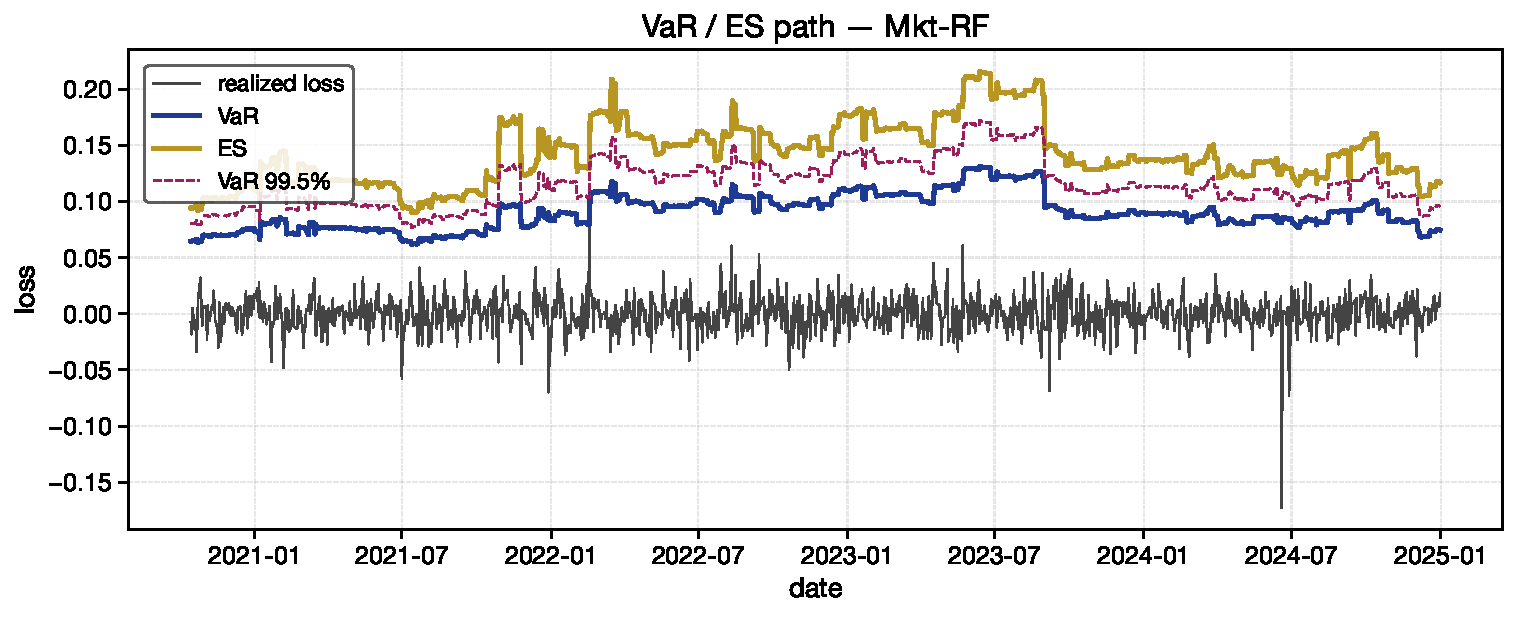
\includegraphics[width=0.85\linewidth]{figures/F9_var_path.pdf}
\caption[Single-portfolio rolling VaR/ES path]{Per-portfolio realised loss (grey), VaR (blue), ES (gold) at the 99\% level, with the 99.5\% VaR overlaid (dashed). Rolling 400-day window. ES sits above VaR throughout; both rise during stress.}
\label{fig:var-path}
\end{figure}


\Cref{fig:var-path} resolves the dashboard of
\cref{fig:var-es-dashboard-placeholder} to a single portfolio (Mkt-RF
in the shipped configuration). The 99\% and 99.5\% VaR paths are
overlaid alongside the realised loss series. The ES curve at the
respective level sits above the VaR curve at every date by
construction.

\begin{figure}[t]
\centering
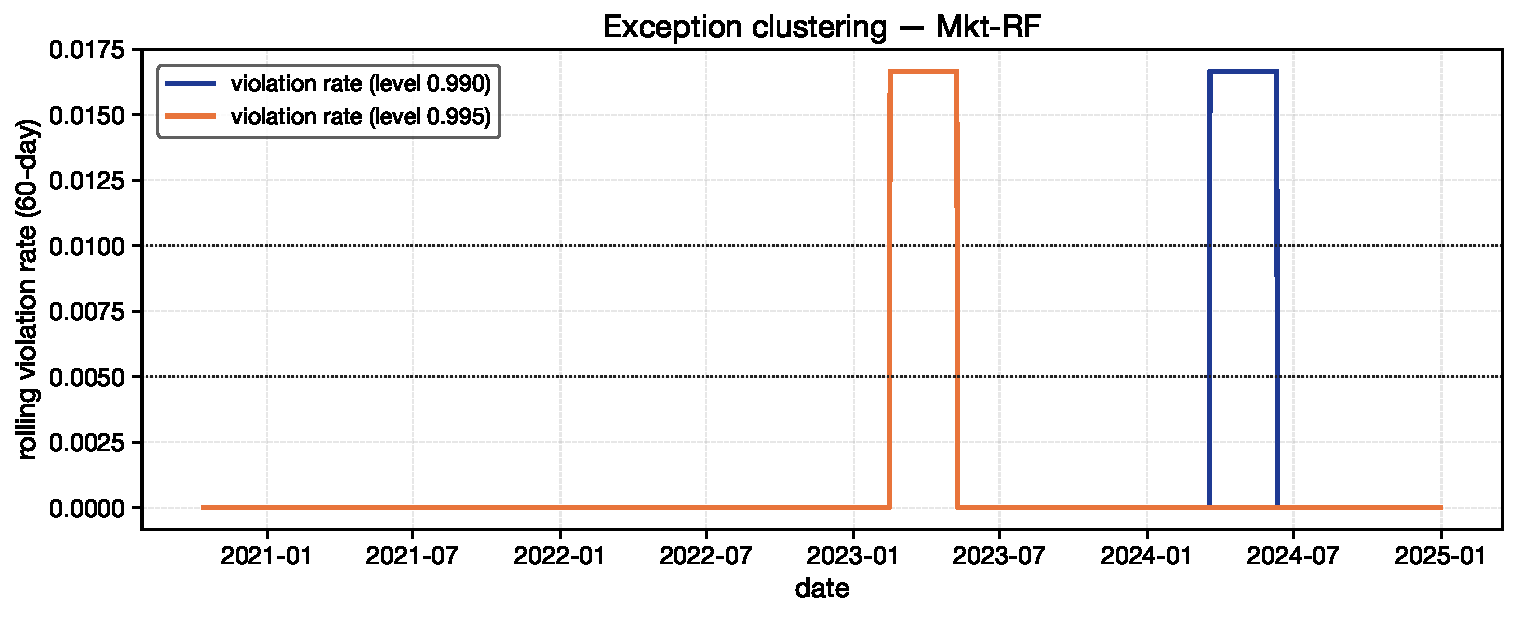
\includegraphics[width=0.85\linewidth]{figures/F10_backtest.pdf}
\caption[Rolling-window exception rate]{Rolling 60-day violation rate of the VaR forecast vs the nominal target level ($1 - \tau$, dotted). Clusters above the target line are evidence of regime changes or model misspecification.}
\label{fig:backtest}
\end{figure}


\Cref{fig:backtest} reports the rolling 60-day exception rate against
the nominal $1 - \tau$ target line. A persistent excursion above the
target is the first signal of regime change or model
misspecification; the dashboard ties this signal to the formal
Kupiec~\cite{Kupiec1995} and Christoffersen~\cite{Christoffersen1998}
tests summarised in \cref{tab:var-es-backtest-placeholder}.

%==============================================================================
% figures/F17_spectral_by_period_placeholder.tex --- Implementation placeholder
%==============================================================================
% Required source CSV: results/F17_spectral_by_period.csv
% Required columns: period, theta_1, theta_2, theta_3, weight, stress_flag
% Replacement instruction: generate a PDF with this basename and replace this
% tikzpicture by an includegraphics command, preserving caption and label.
%==============================================================================
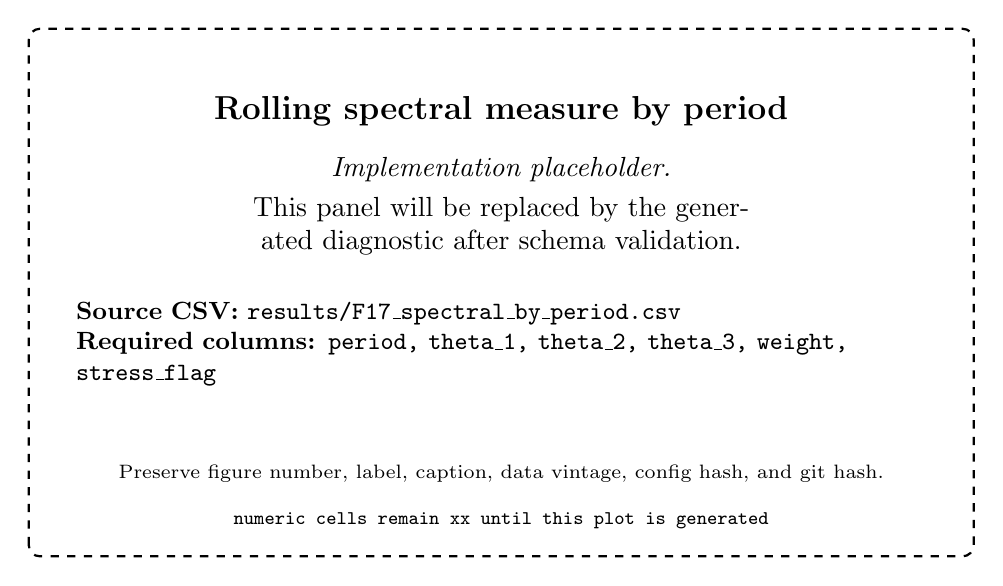
\begin{tikzpicture}
\draw[thick, dashed, rounded corners] (0,0) rectangle (12,6.7);
\node[align=center, font=\large] at (6,5.65) {\textbf{Rolling spectral measure by period}};
\node[align=center, text width=10.6cm] at (6,4.45) {\emph{Implementation placeholder.}\\[0.25em]
This panel will be replaced by the generated diagnostic after schema validation.};
\node[align=left, text width=10.8cm, font=\small] at (6,2.7) {\textbf{Source CSV:} \texttt{results/F17\_spectral\_by\_period.csv}\\
\textbf{Required columns:} \texttt{period, theta\_1, theta\_2, theta\_3, weight, stress\_flag}};
\node[align=center, font=\scriptsize] at (6,1.05) {Preserve figure number, label, caption, data vintage, config hash, and git hash.};
\node[align=center, font=\scriptsize\ttfamily] at (6,0.45) {numeric cells remain xx until this plot is generated};
\end{tikzpicture}


\Cref{fig:spectral-by-period-placeholder} reports the empirical
angular mass per real factor across three rolling periods. On a
stationary panel the three bars per factor are nearly identical; on
live FF data a regime-change window (e.g.\ the 2007--09 GFC) would
show pronounced mass migration onto the market factor, consistent with
the "in stress, everything is the market" finding of
\citet{ChristoffersenErrunzaJacobsLangloi2012}.
